\documentclass[12pt, a4paper]{article}\usepackage[]{graphicx}\usepackage[]{color}
%% maxwidth is the original width if it is less than linewidth
%% otherwise use linewidth (to make sure the graphics do not exceed the margin)
\makeatletter
\def\maxwidth{ %
  \ifdim\Gin@nat@width>\linewidth
    \linewidth
  \else
    \Gin@nat@width
  \fi
}
\makeatother

\definecolor{fgcolor}{rgb}{0.345, 0.345, 0.345}
\newcommand{\hlnum}[1]{\textcolor[rgb]{0.686,0.059,0.569}{#1}}%
\newcommand{\hlstr}[1]{\textcolor[rgb]{0.192,0.494,0.8}{#1}}%
\newcommand{\hlcom}[1]{\textcolor[rgb]{0.678,0.584,0.686}{\textit{#1}}}%
\newcommand{\hlopt}[1]{\textcolor[rgb]{0,0,0}{#1}}%
\newcommand{\hlstd}[1]{\textcolor[rgb]{0.345,0.345,0.345}{#1}}%
\newcommand{\hlkwa}[1]{\textcolor[rgb]{0.161,0.373,0.58}{\textbf{#1}}}%
\newcommand{\hlkwb}[1]{\textcolor[rgb]{0.69,0.353,0.396}{#1}}%
\newcommand{\hlkwc}[1]{\textcolor[rgb]{0.333,0.667,0.333}{#1}}%
\newcommand{\hlkwd}[1]{\textcolor[rgb]{0.737,0.353,0.396}{\textbf{#1}}}%
\let\hlipl\hlkwb

\usepackage{framed}
\makeatletter
\newenvironment{kframe}{%
 \def\at@end@of@kframe{}%
 \ifinner\ifhmode%
  \def\at@end@of@kframe{\end{minipage}}%
  \begin{minipage}{\columnwidth}%
 \fi\fi%
 \def\FrameCommand##1{\hskip\@totalleftmargin \hskip-\fboxsep
 \colorbox{shadecolor}{##1}\hskip-\fboxsep
     % There is no \\@totalrightmargin, so:
     \hskip-\linewidth \hskip-\@totalleftmargin \hskip\columnwidth}%
 \MakeFramed {\advance\hsize-\width
   \@totalleftmargin\z@ \linewidth\hsize
   \@setminipage}}%
 {\par\unskip\endMakeFramed%
 \at@end@of@kframe}
\makeatother

\definecolor{shadecolor}{rgb}{.97, .97, .97}
\definecolor{messagecolor}{rgb}{0, 0, 0}
\definecolor{warningcolor}{rgb}{1, 0, 1}
\definecolor{errorcolor}{rgb}{1, 0, 0}
\newenvironment{knitrout}{}{} % an empty environment to be redefined in TeX

\usepackage{alltt}
\usepackage[utf8]{inputenc}
\usepackage{longtable}
\usepackage{multirow} 
\usepackage{hyperref}
\usepackage[titles]{tocloft}
\usepackage[affil-it]{authblk}


\setlength\parindent{0pt}

\title{\textbf{\Large Alignment Stats}}

\author {Lucas Michel Todó, Cristina Bancells\\
Alfred Cortes and Juan R. Gonzalez}

\affil{Barcelona Global Health Institute (ISGlobal), Campus PRBB}
\IfFileExists{upquote.sty}{\usepackage{upquote}}{}
\begin{document}
	
\maketitle
\tableofcontents
\newpage



\section{Importing Data}

First we import the data for every alignment:
\begin{knitrout}
\definecolor{shadecolor}{rgb}{0.969, 0.969, 0.969}\color{fgcolor}\begin{kframe}
\begin{alltt}
\hlcom{####  Fetch files and create iterables ####}
\hlstd{file_names} \hlkwb{<-} \hlkwd{list.files}\hlstd{(}\hlstr{"/home/lucas/ISGlobal/TestSet/align_tests/inputs/"}\hlstd{)}
\hlstd{file_names} \hlkwb{<-} \hlkwd{unique}\hlstd{(}\hlkwd{lapply}\hlstd{(file_names,} \hlkwa{function}\hlstd{(}\hlkwc{x}\hlstd{)} \hlkwd{substr}\hlstd{(x,}\hlnum{1}\hlstd{,}\hlnum{17}\hlstd{)))}

\hlstd{dirs} \hlkwb{<-} \hlkwd{list.files}\hlstd{(}\hlstr{"/home/lucas/ISGlobal/TestSet/align_tests/"}\hlstd{)[}\hlkwd{substr}\hlstd{(}\hlkwd{list.files}\hlstd{(}\hlstr{"/home/lucas/ISGlobal/TestSet/align_tests/"}\hlstd{),}\hlnum{1}\hlstd{,}\hlnum{6}\hlstd{)} \hlopt{==} \hlstr{"params"}\hlstd{]}
\end{alltt}
\end{kframe}
\end{knitrout}

\section{Plots}
\subsection{MAPQ}

\begin{knitrout}
\definecolor{shadecolor}{rgb}{0.969, 0.969, 0.969}\color{fgcolor}\begin{kframe}
\begin{alltt}
\hlkwa{for} \hlstd{(dir} \hlkwa{in} \hlstd{dirs)\{}
  \hlkwa{for} \hlstd{(x} \hlkwa{in} \hlstd{file_names)\{}
    \hlstd{mapq} \hlkwb{<-} \hlkwd{read.csv2}\hlstd{(}\hlkwc{file} \hlstd{=} \hlkwd{paste0}\hlstd{(}\hlstr{"/home/lucas/ISGlobal/TestSet/align_tests/"}\hlstd{,dir,}\hlstr{"/"}\hlstd{,x,}\hlstr{"_MAPQ.csv"}\hlstd{),} \hlkwc{sep} \hlstd{=} \hlstr{"\textbackslash{}t"}\hlstd{,} \hlkwc{header} \hlstd{=} \hlnum{FALSE}\hlstd{)}
    \hlstd{df} \hlkwb{<-} \hlkwd{as.data.frame}\hlstd{(}\hlkwd{as.numeric}\hlstd{(mapq))}
    \hlkwd{colnames}\hlstd{(df)} \hlkwb{<-} \hlstr{"MAPQ"}
    \hlstd{title} \hlkwb{<-} \hlstd{x}
    \hlkwd{print}\hlstd{(}\hlkwd{ggplot}\hlstd{(df,} \hlkwd{aes}\hlstd{(}\hlkwc{x} \hlstd{= MAPQ))} \hlopt{+}
        \hlkwd{geom_histogram}\hlstd{(}\hlkwc{binwidth} \hlstd{=} \hlnum{1}\hlstd{)} \hlopt{+}
        \hlkwd{labs}\hlstd{(}\hlkwc{x} \hlstd{=} \hlstr{"MAPQ"}\hlstd{,} \hlkwc{y} \hlstd{=} \hlstr{"Count"}\hlstd{)} \hlopt{+}
        \hlkwd{ggtitle}\hlstd{(title)} \hlopt{+}
        \hlkwd{theme}\hlstd{(}\hlkwc{plot.title} \hlstd{=} \hlkwd{element_text}\hlstd{(}\hlkwc{hjust} \hlstd{=} \hlnum{0.5}\hlstd{))} \hlopt{+}
        \hlkwd{scale_x_continuous}\hlstd{(}\hlkwc{breaks} \hlstd{=} \hlkwd{seq}\hlstd{(}\hlnum{0}\hlstd{,} \hlnum{45}\hlstd{,} \hlkwc{by} \hlstd{=} \hlnum{2}\hlstd{),} \hlkwc{limits} \hlstd{=} \hlkwd{c}\hlstd{(}\hlnum{0}\hlstd{,}\hlnum{48}\hlstd{))} \hlopt{+}
        \hlkwd{scale_y_continuous}\hlstd{(}\hlkwc{breaks} \hlstd{=} \hlkwd{seq}\hlstd{(}\hlnum{0}\hlstd{,}\hlnum{80000}\hlstd{,} \hlkwc{by} \hlstd{=} \hlnum{5000}\hlstd{)))}

    \hlkwd{plot.new}\hlstd{()}
    \hlkwd{print}\hlstd{(}\hlkwd{table}\hlstd{(df} \hlopt{>} \hlnum{5}\hlstd{))}
  \hlstd{\}}
\hlstd{\}}
\end{alltt}
\end{kframe}
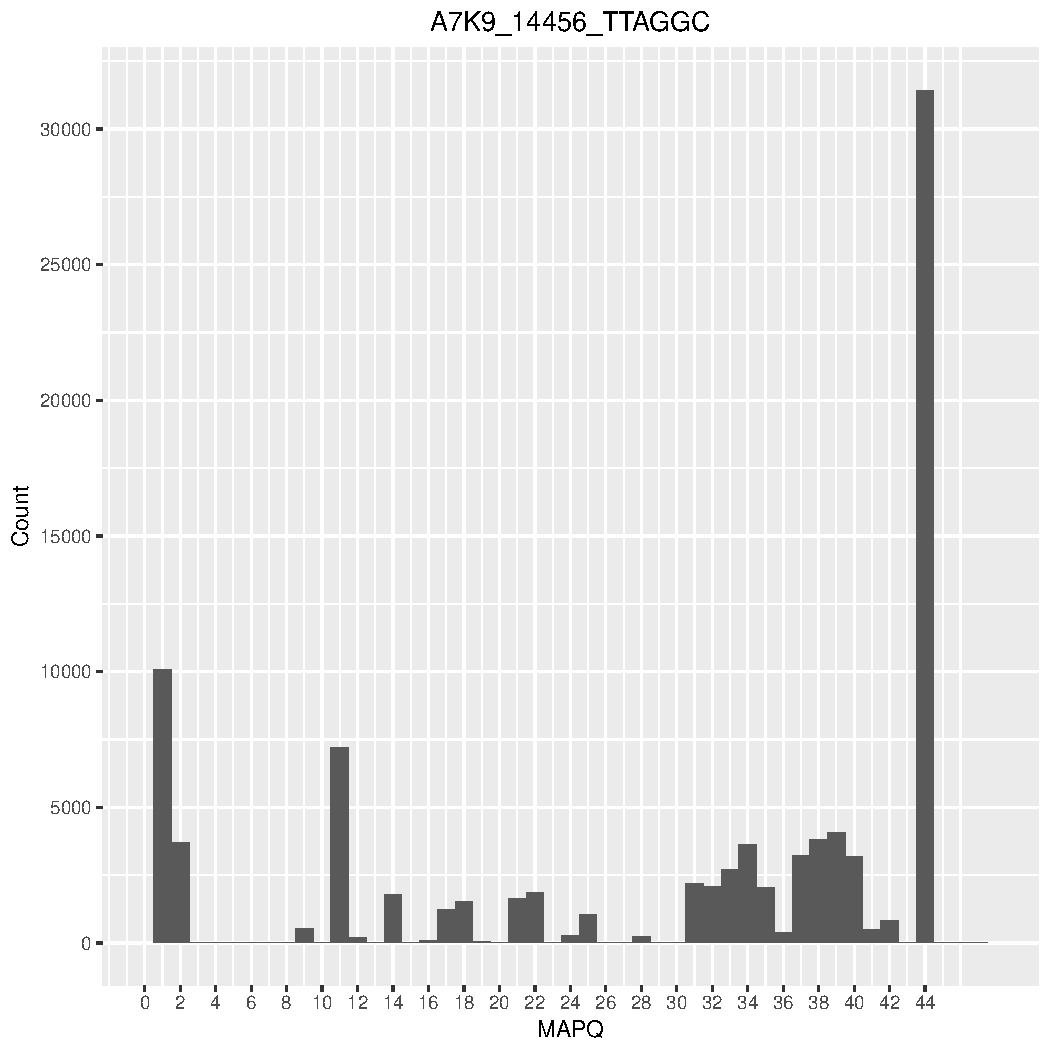
\includegraphics[width=\maxwidth]{figure/unnamed-chunk-3-1} 


\includegraphics[width=\maxwidth]{figure/unnamed-chunk-3-2} 
\begin{kframe}\begin{verbatim}
## 
## FALSE  TRUE 
## 32237 77763
\end{verbatim}
\end{kframe}
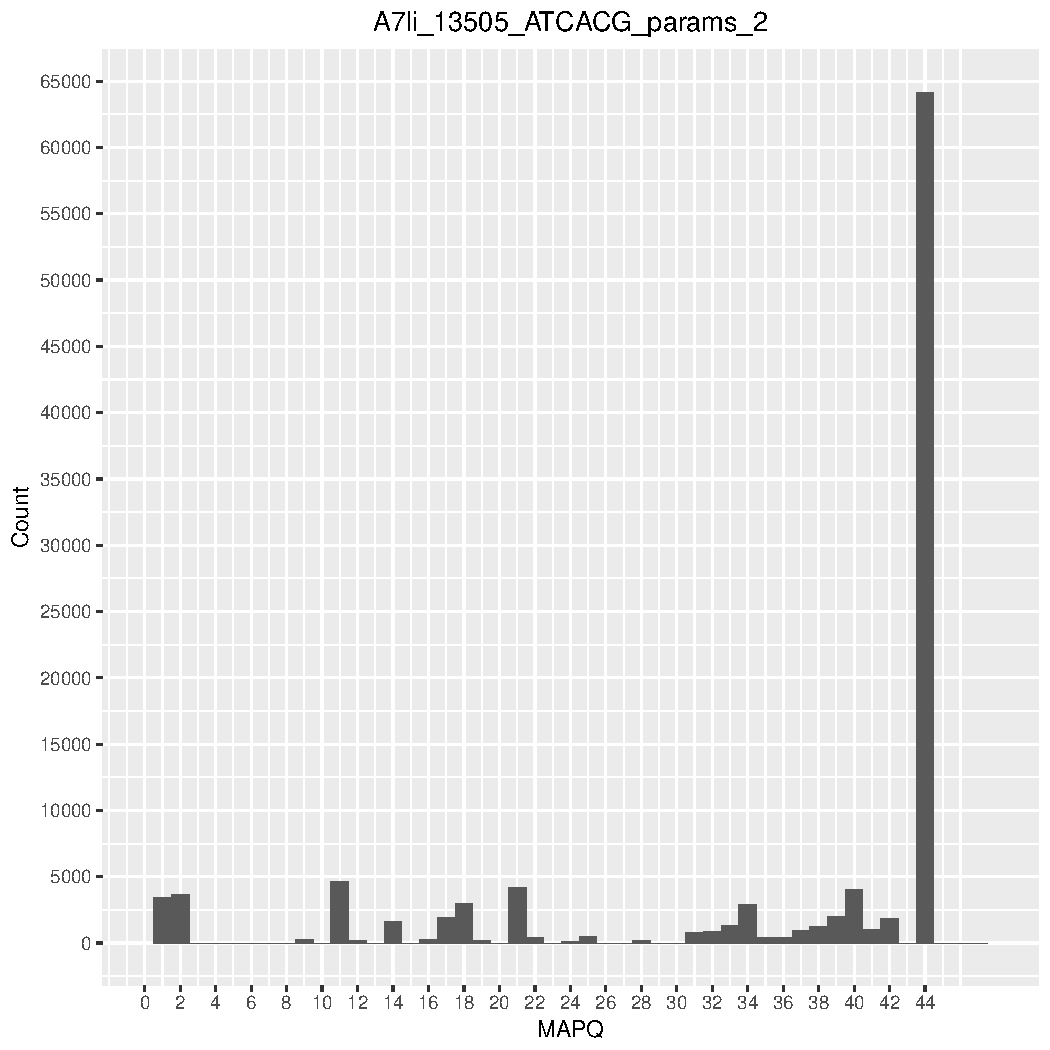
\includegraphics[width=\maxwidth]{figure/unnamed-chunk-3-3} 

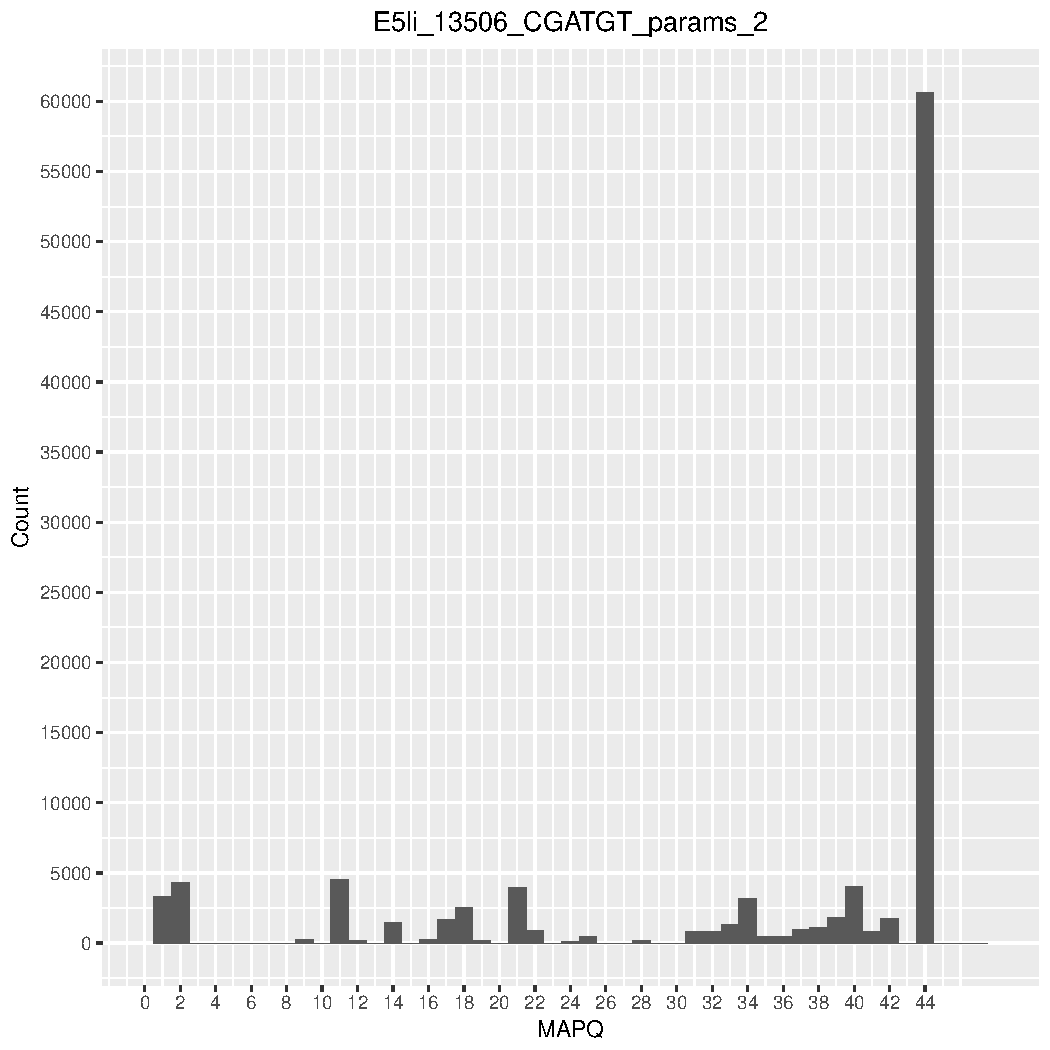
\includegraphics[width=\maxwidth]{figure/unnamed-chunk-3-4} 
\begin{kframe}\begin{verbatim}
## 
## FALSE  TRUE 
## 10747 99253
\end{verbatim}
\end{kframe}
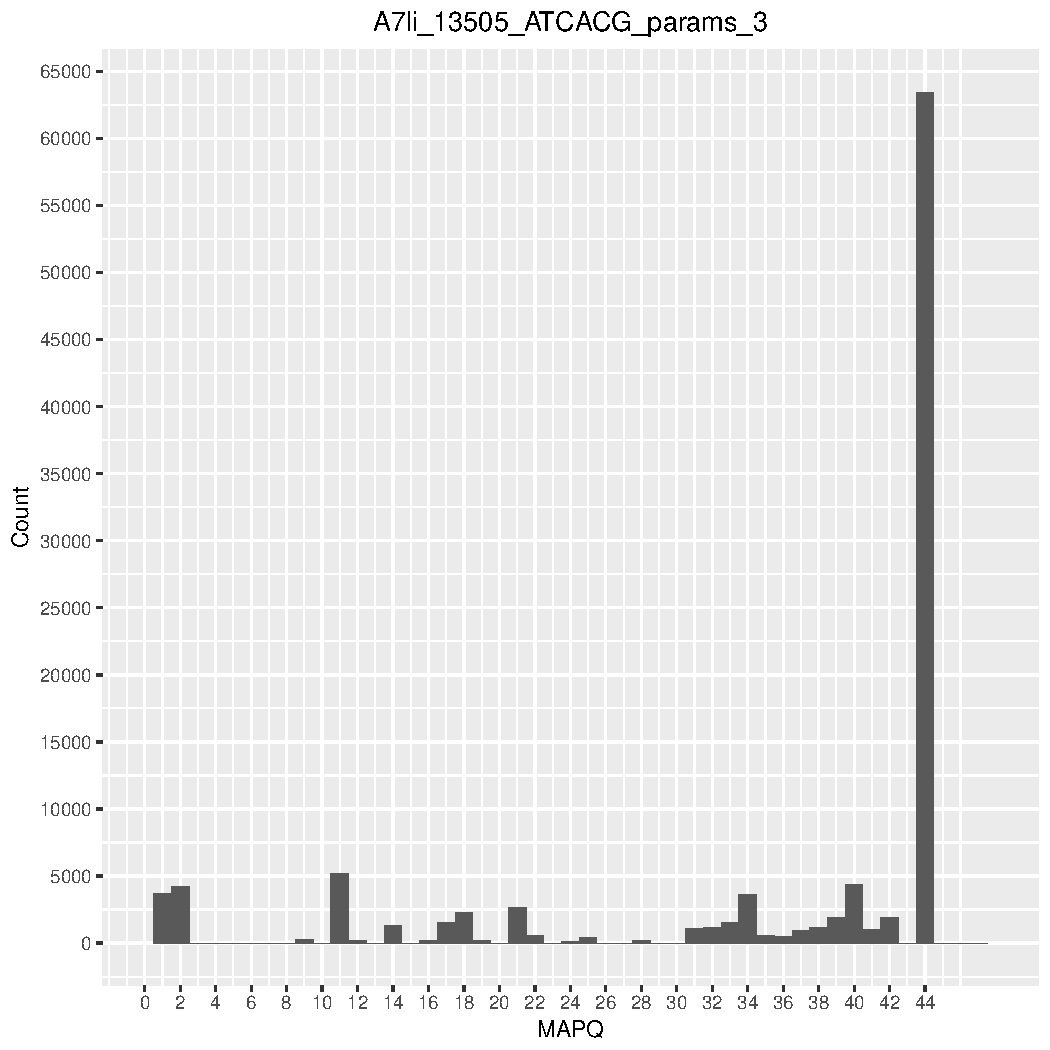
\includegraphics[width=\maxwidth]{figure/unnamed-chunk-3-5} 

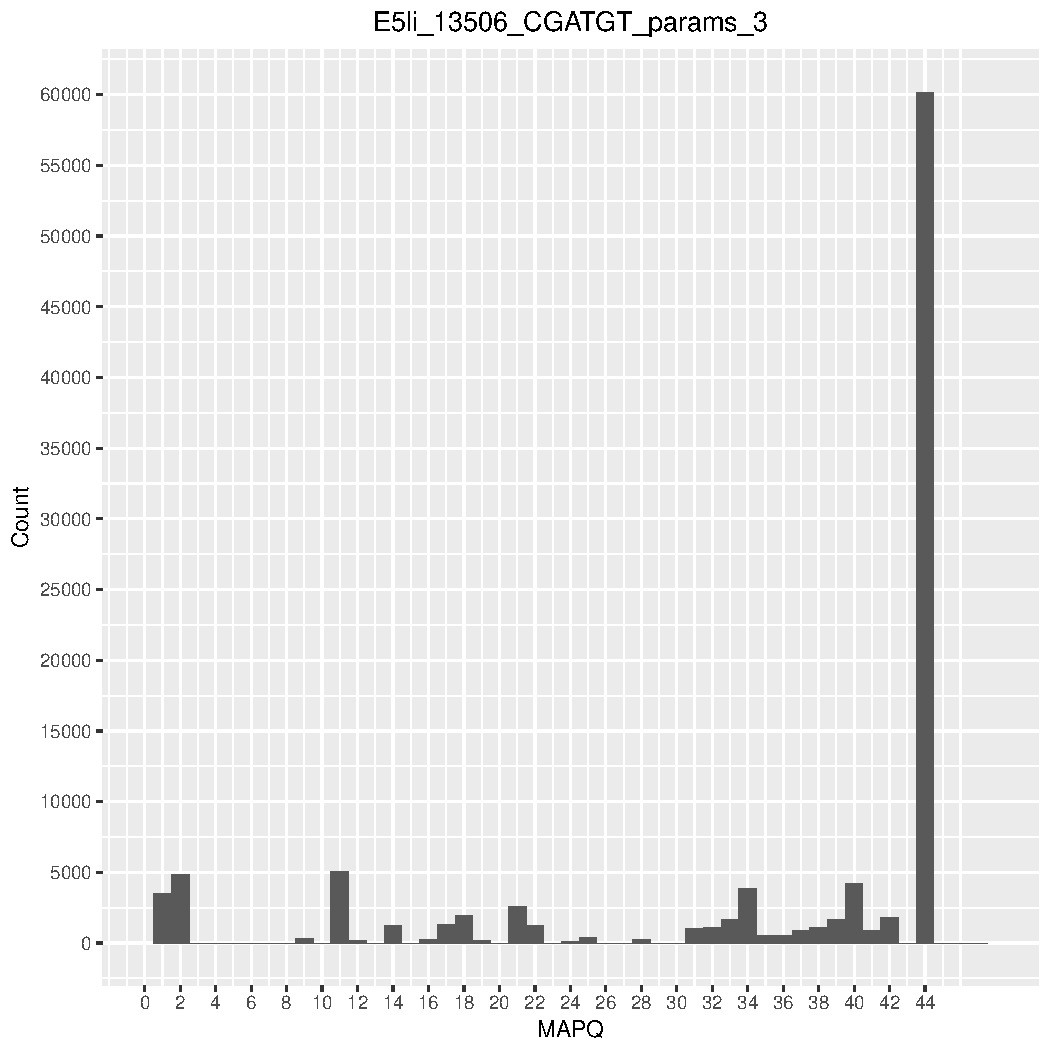
\includegraphics[width=\maxwidth]{figure/unnamed-chunk-3-6} 
\begin{kframe}\begin{verbatim}
## 
## FALSE  TRUE 
## 36833 73167
\end{verbatim}
\end{kframe}
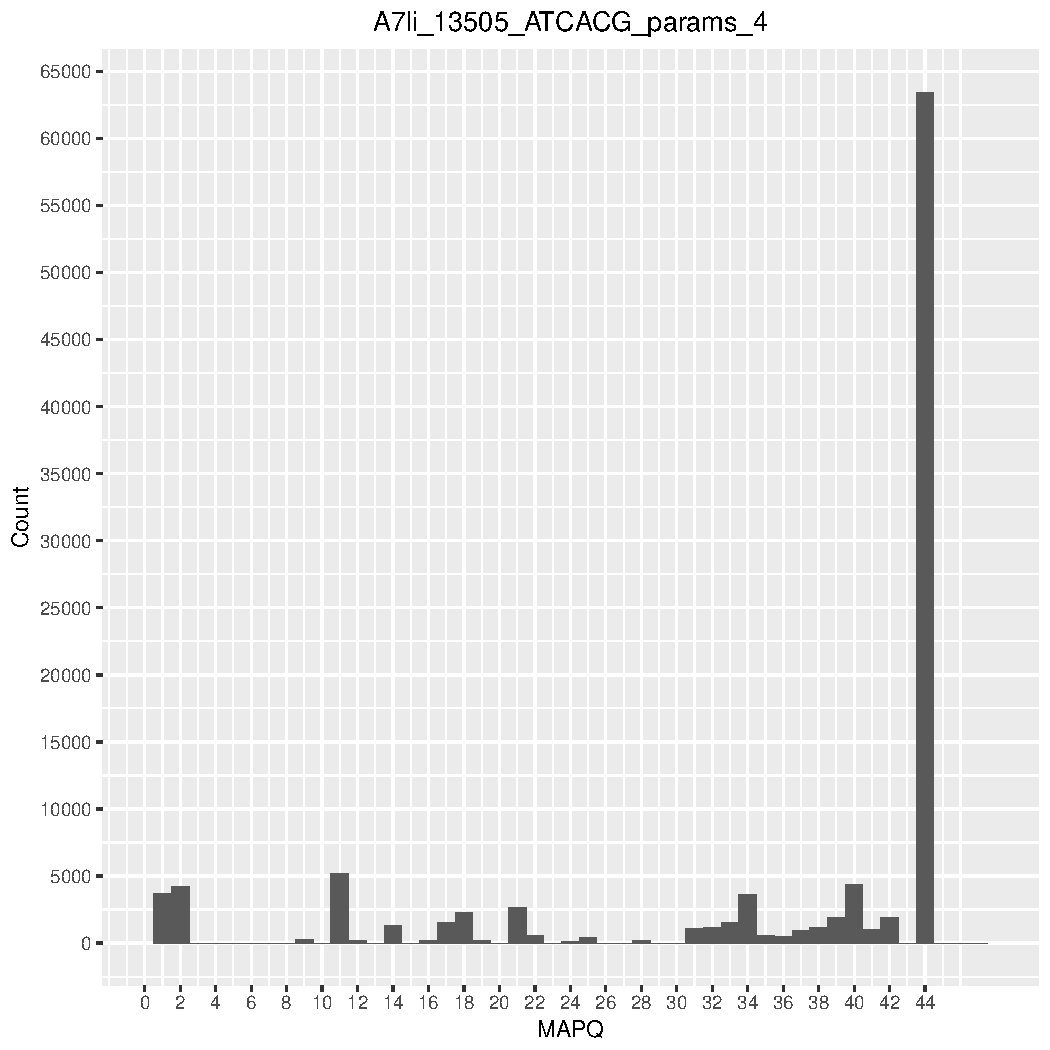
\includegraphics[width=\maxwidth]{figure/unnamed-chunk-3-7} 

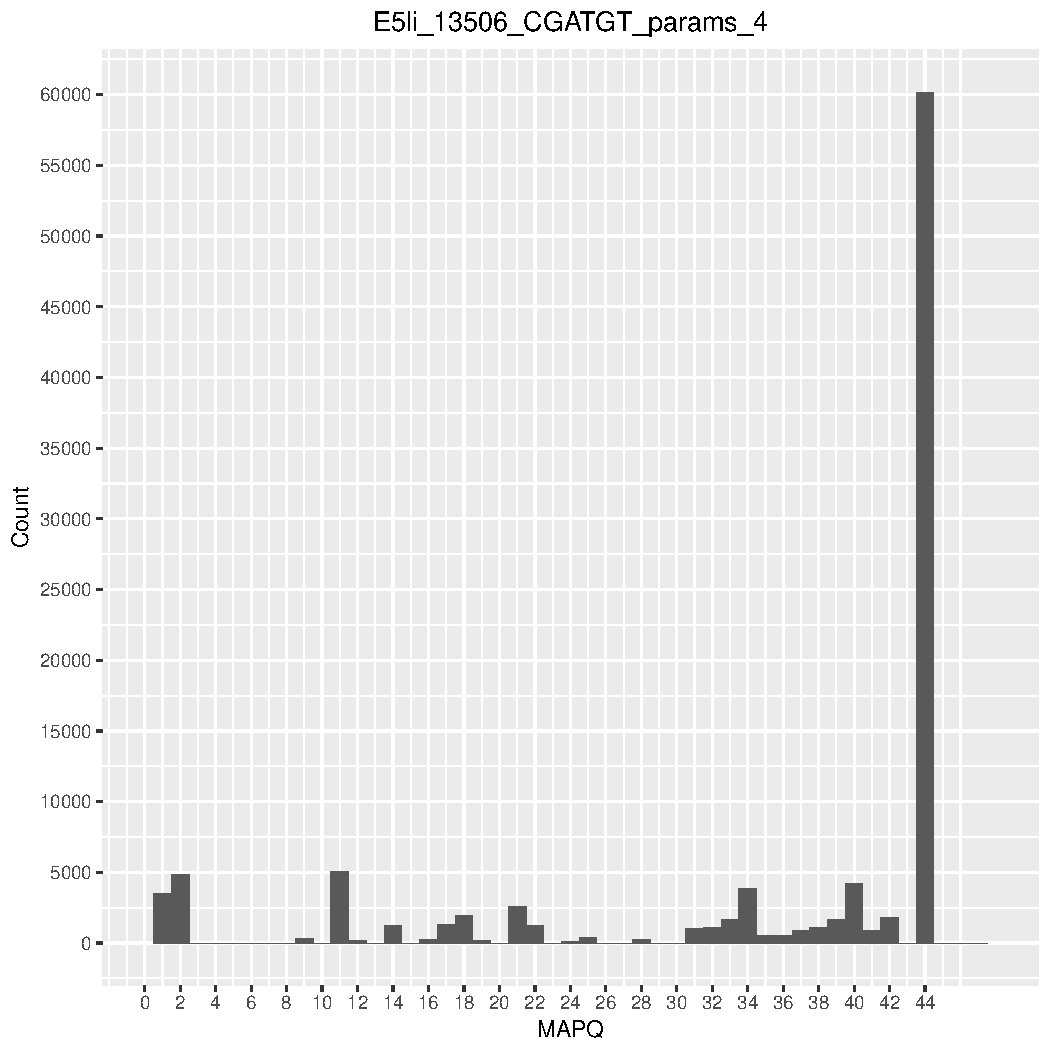
\includegraphics[width=\maxwidth]{figure/unnamed-chunk-3-8} 
\begin{kframe}\begin{verbatim}
## 
## FALSE  TRUE 
##  2265     5
\end{verbatim}
\end{kframe}
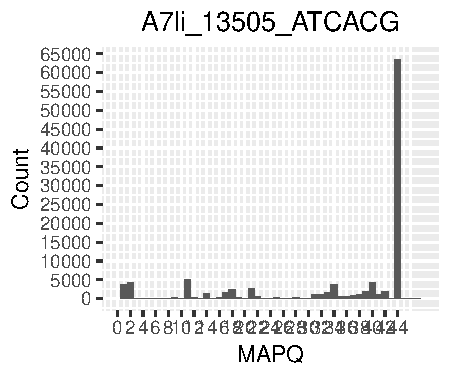
\includegraphics[width=\maxwidth]{figure/unnamed-chunk-3-9} 


\includegraphics[width=\maxwidth]{figure/unnamed-chunk-3-10} 
\begin{kframe}\begin{verbatim}
## 
## FALSE  TRUE 
## 15355 94645
\end{verbatim}
\end{kframe}
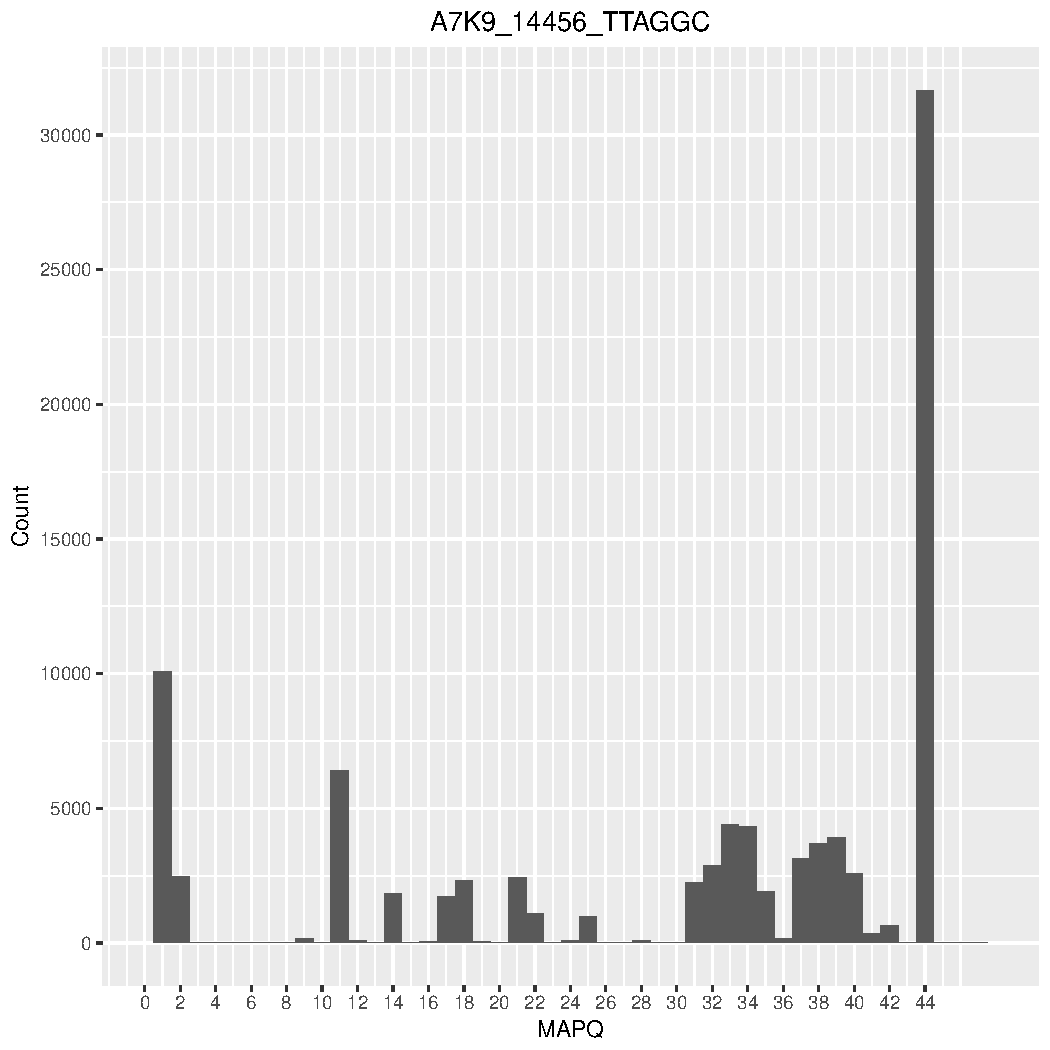
\includegraphics[width=\maxwidth]{figure/unnamed-chunk-3-11} 


\includegraphics[width=\maxwidth]{figure/unnamed-chunk-3-12} 
\begin{kframe}\begin{verbatim}
## 
## FALSE  TRUE 
## 30779 79221
\end{verbatim}
\end{kframe}
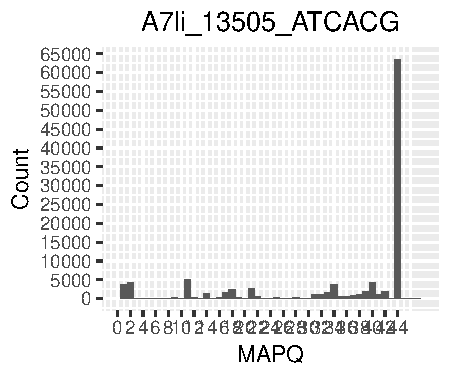
\includegraphics[width=\maxwidth]{figure/unnamed-chunk-3-13} 


\includegraphics[width=\maxwidth]{figure/unnamed-chunk-3-14} 
\begin{kframe}\begin{verbatim}
## 
## FALSE  TRUE 
## 10396 99604
\end{verbatim}
\end{kframe}
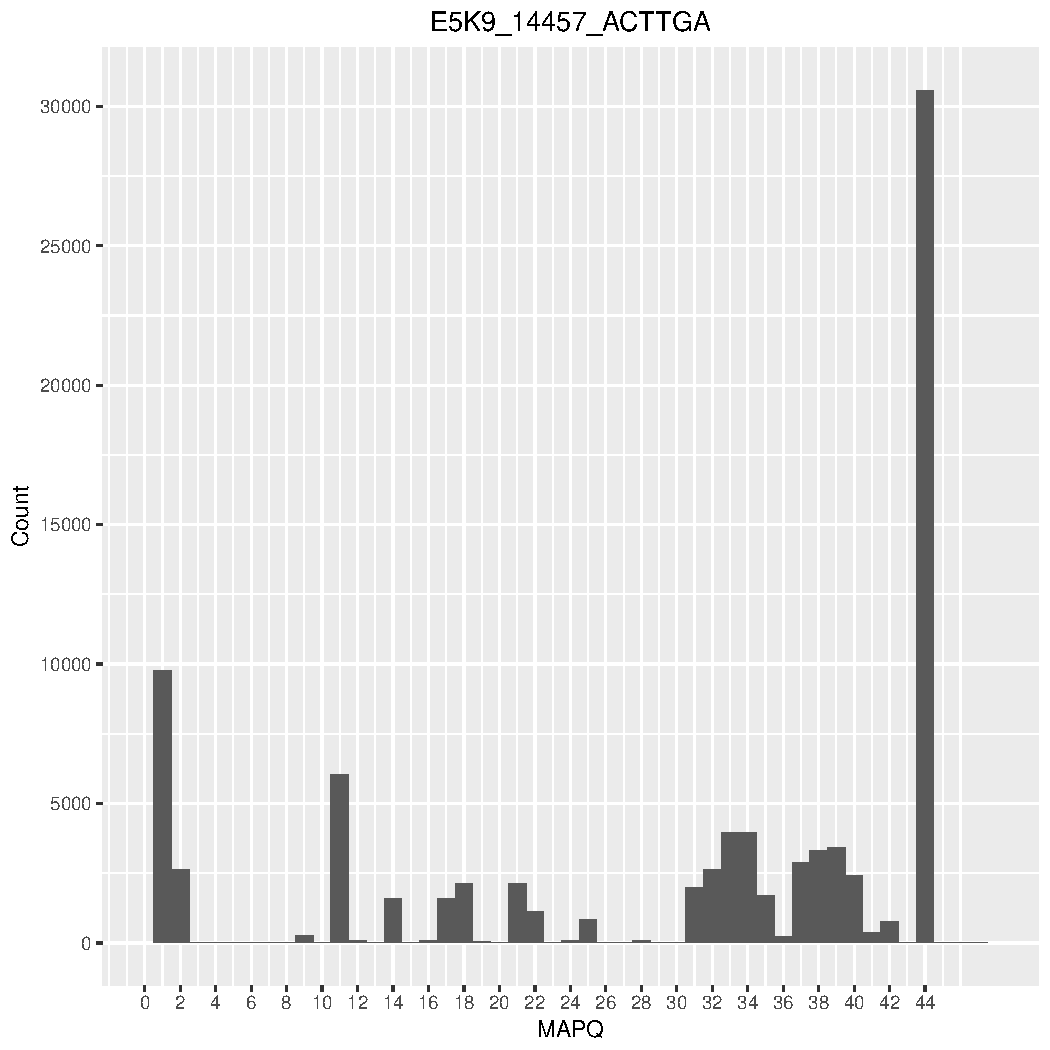
\includegraphics[width=\maxwidth]{figure/unnamed-chunk-3-15} 


\includegraphics[width=\maxwidth]{figure/unnamed-chunk-3-16} 
\begin{kframe}\begin{verbatim}
## 
## FALSE  TRUE 
## 35707 74293
\end{verbatim}
\end{kframe}
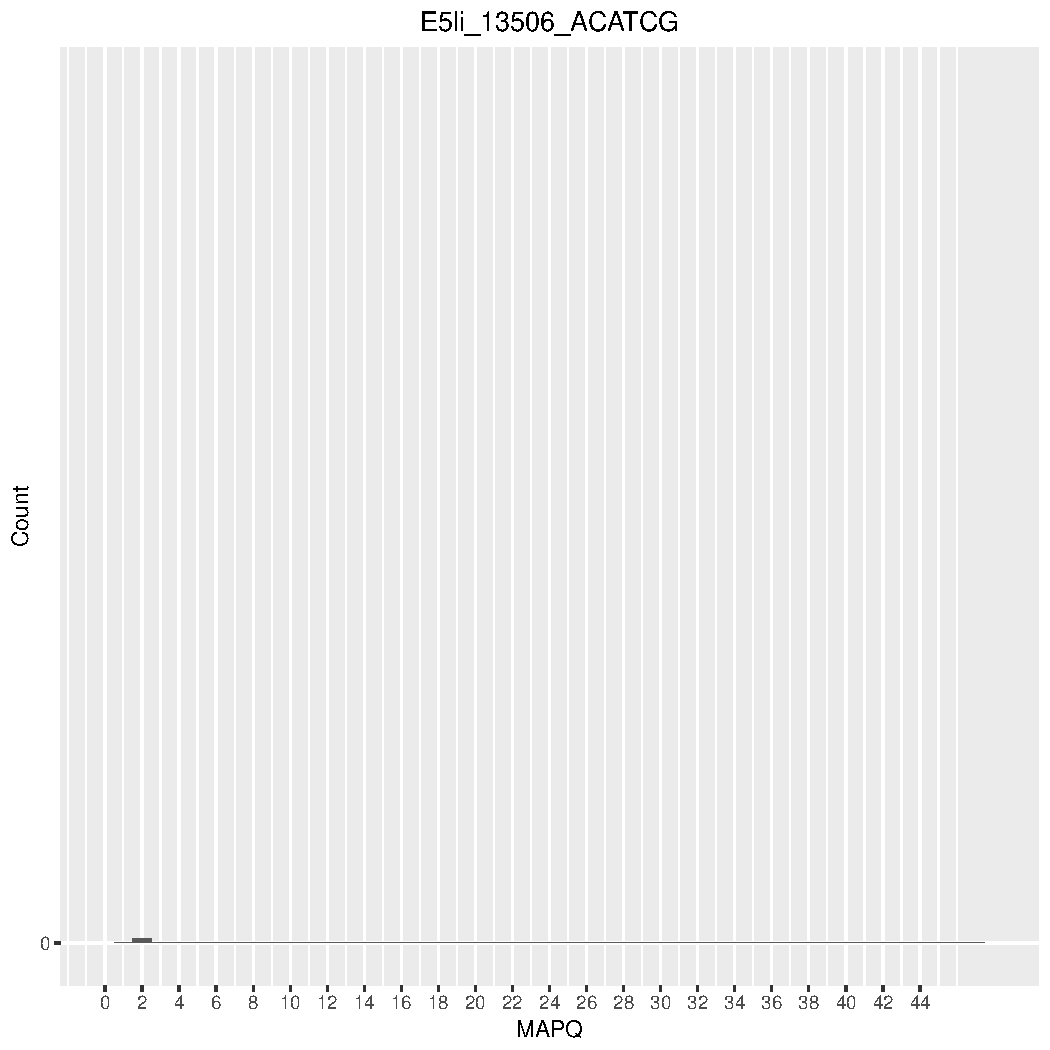
\includegraphics[width=\maxwidth]{figure/unnamed-chunk-3-17} 


\includegraphics[width=\maxwidth]{figure/unnamed-chunk-3-18} 
\begin{kframe}\begin{verbatim}
## 
## FALSE  TRUE 
##  2265     5
\end{verbatim}
\end{kframe}
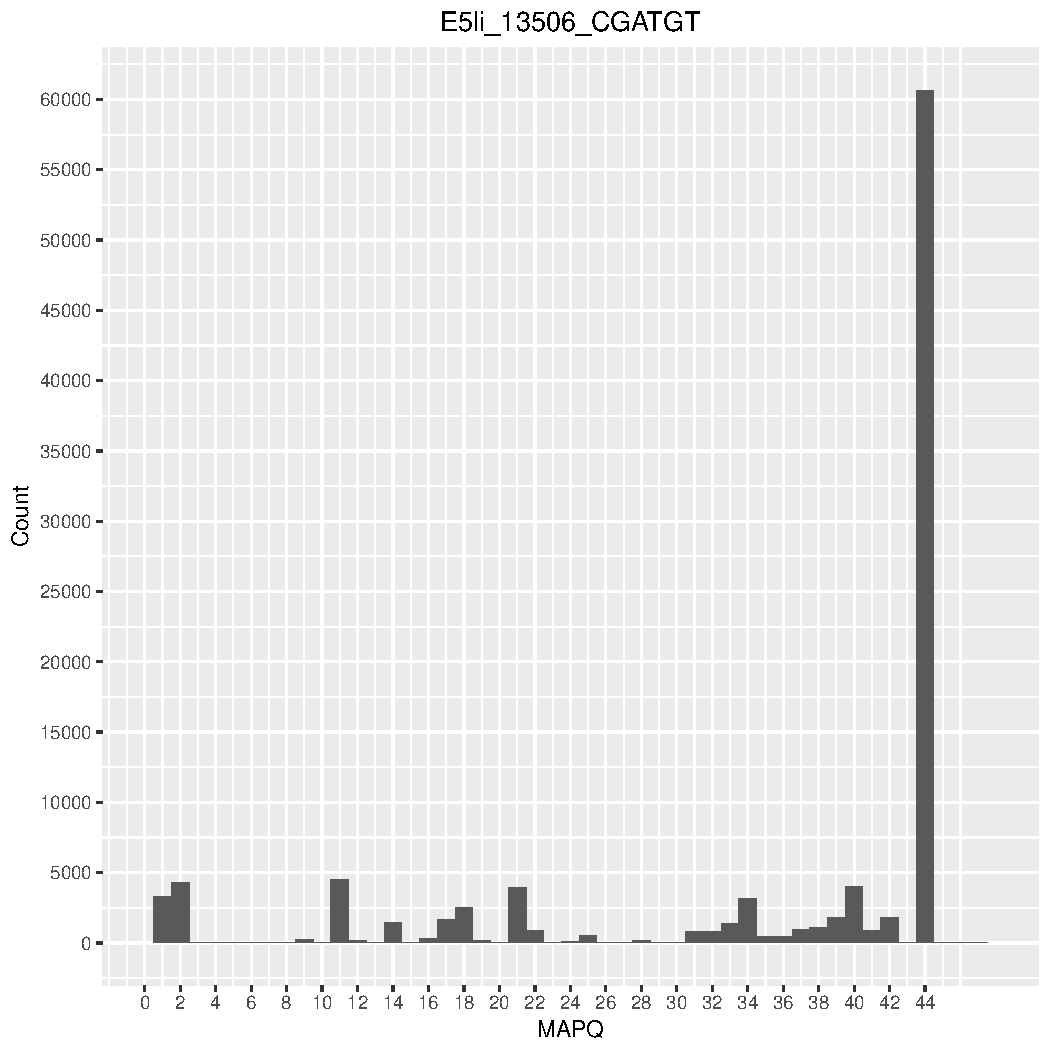
\includegraphics[width=\maxwidth]{figure/unnamed-chunk-3-19} 


\includegraphics[width=\maxwidth]{figure/unnamed-chunk-3-20} 
\begin{kframe}\begin{verbatim}
## 
## FALSE  TRUE 
## 14955 95045
\end{verbatim}
\end{kframe}
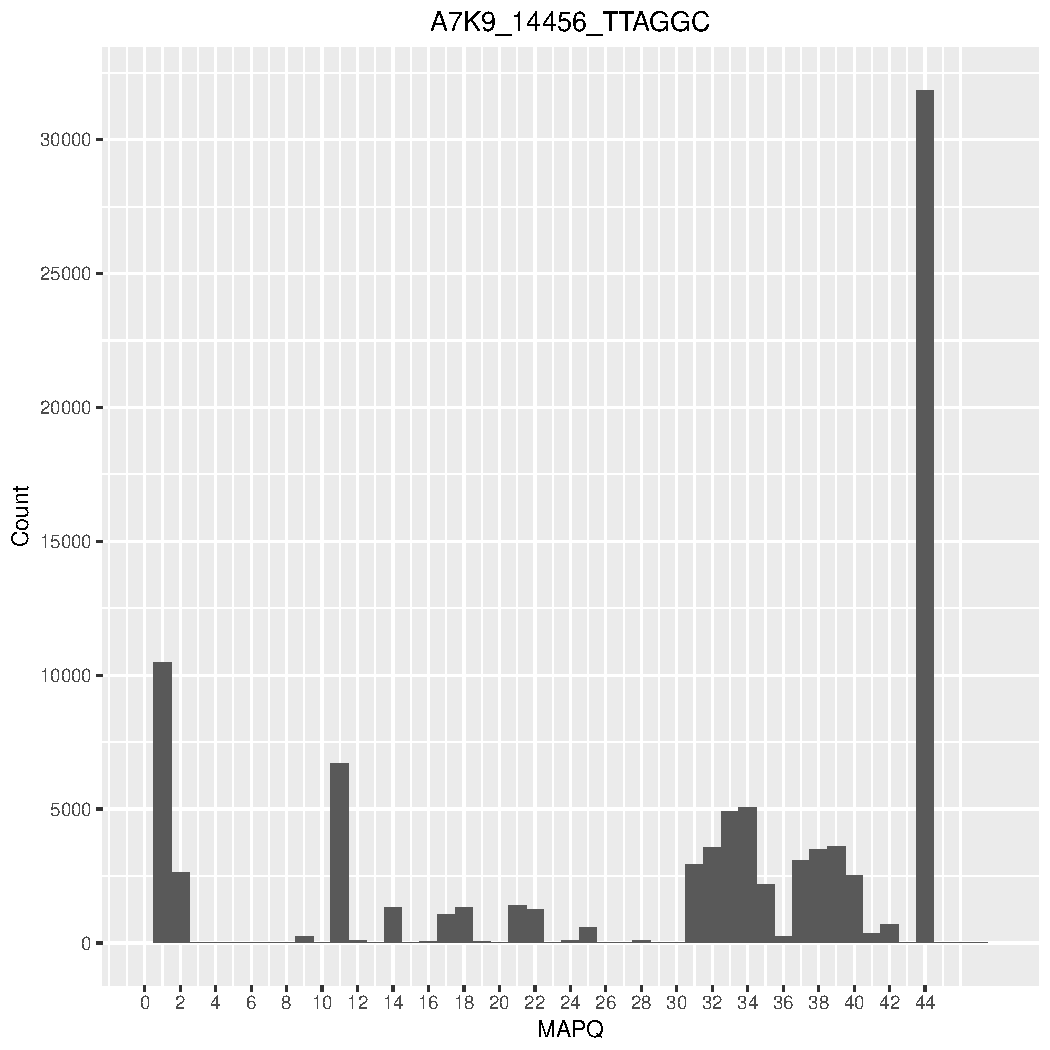
\includegraphics[width=\maxwidth]{figure/unnamed-chunk-3-21} 


\includegraphics[width=\maxwidth]{figure/unnamed-chunk-3-22} 
\begin{kframe}\begin{verbatim}
## 
## FALSE  TRUE 
## 31263 78737
\end{verbatim}
\end{kframe}
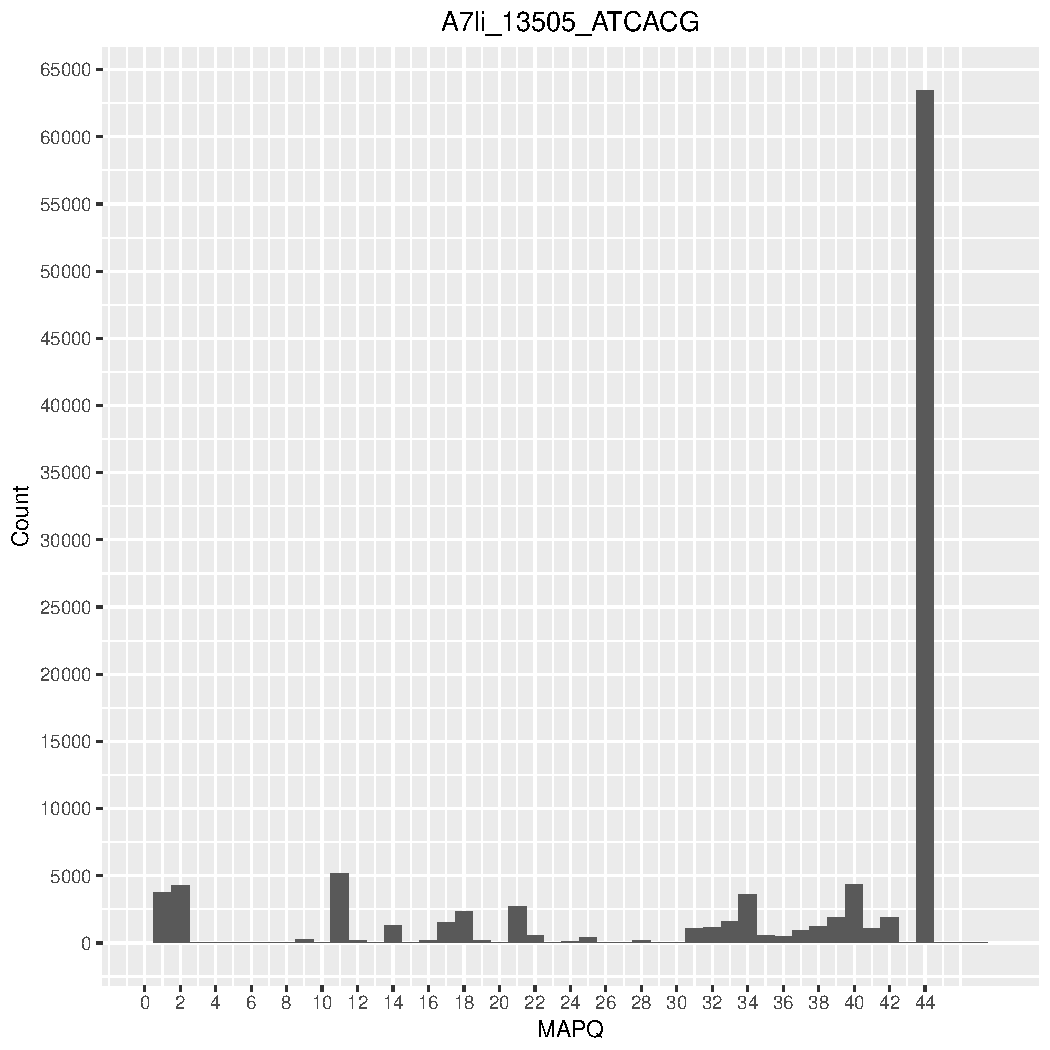
\includegraphics[width=\maxwidth]{figure/unnamed-chunk-3-23} 


\includegraphics[width=\maxwidth]{figure/unnamed-chunk-3-24} 
\begin{kframe}\begin{verbatim}
## 
## FALSE  TRUE 
## 11487 98513
\end{verbatim}
\end{kframe}
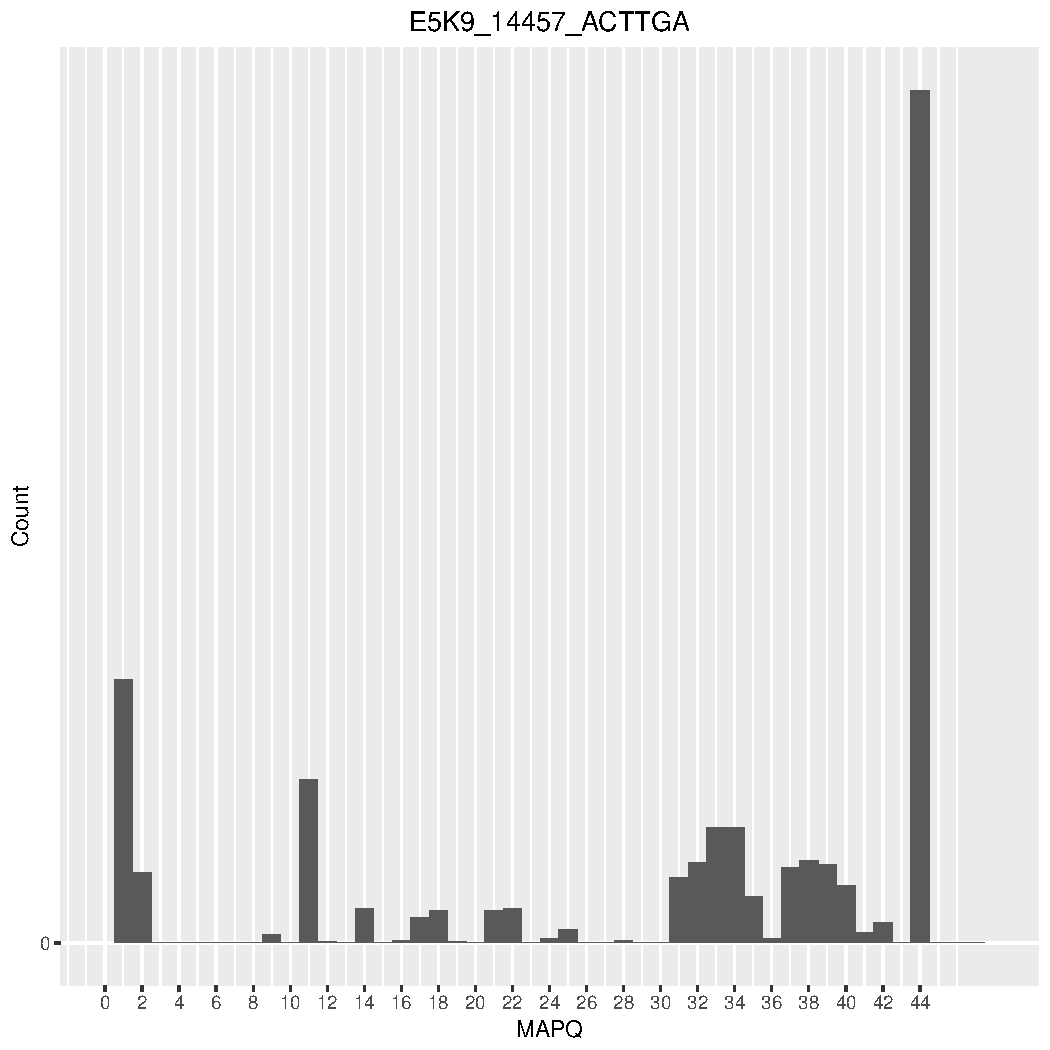
\includegraphics[width=\maxwidth]{figure/unnamed-chunk-3-25} 


\includegraphics[width=\maxwidth]{figure/unnamed-chunk-3-26} 
\begin{kframe}\begin{verbatim}
## 
## FALSE  TRUE 
##  4521  9328
\end{verbatim}
\end{kframe}
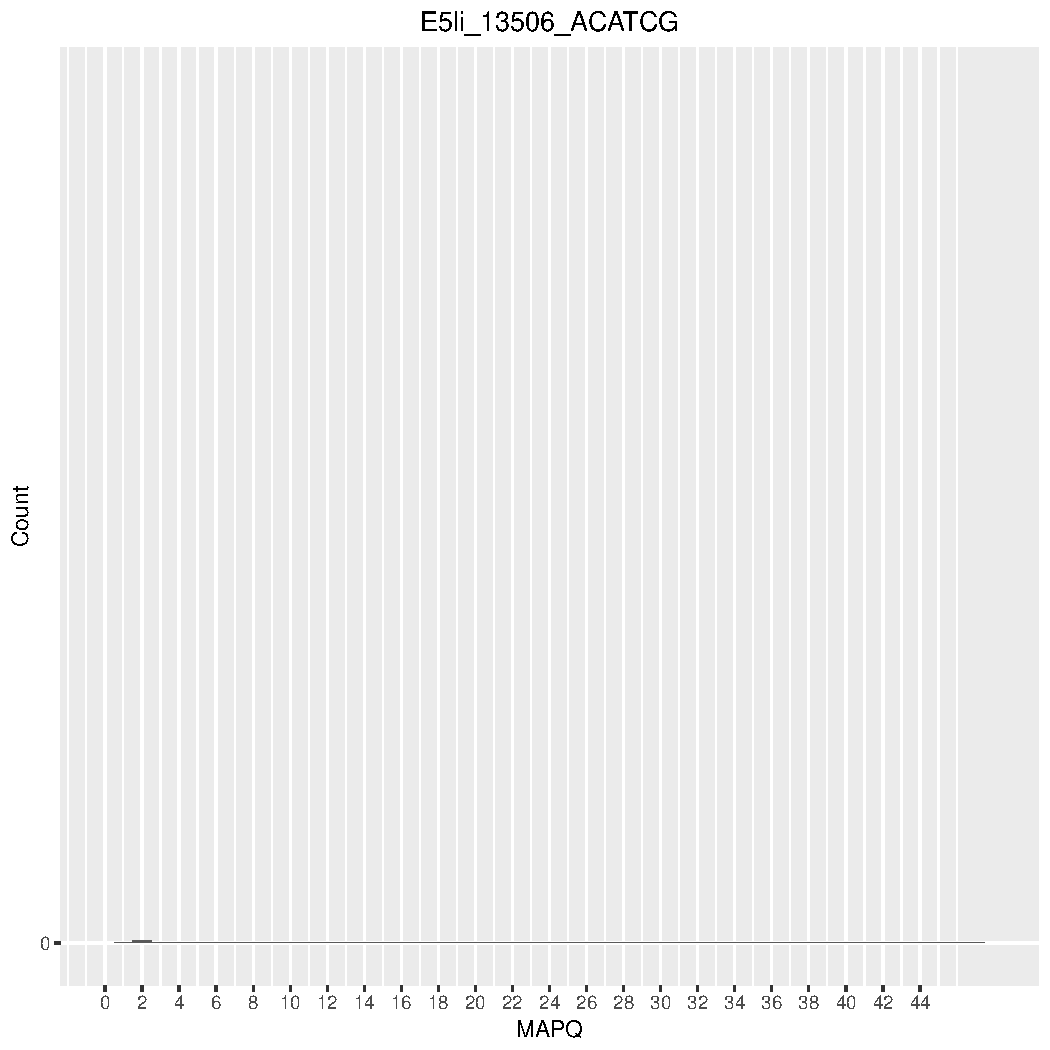
\includegraphics[width=\maxwidth]{figure/unnamed-chunk-3-27} 


\includegraphics[width=\maxwidth]{figure/unnamed-chunk-3-28} 
\begin{kframe}\begin{verbatim}
## 
## FALSE  TRUE 
##  2264     6
\end{verbatim}
\end{kframe}
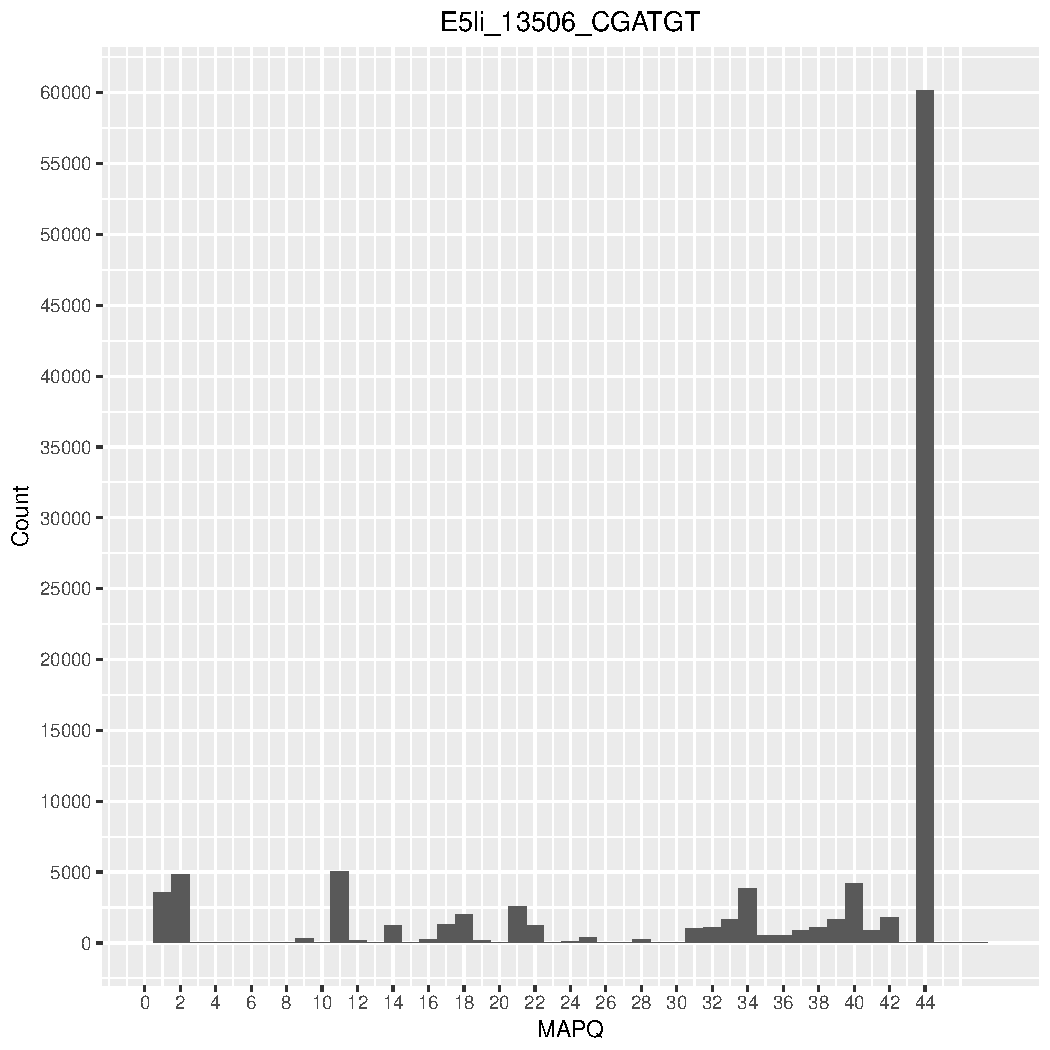
\includegraphics[width=\maxwidth]{figure/unnamed-chunk-3-29} 


\includegraphics[width=\maxwidth]{figure/unnamed-chunk-3-30} 
\begin{kframe}\begin{verbatim}
## 
## FALSE  TRUE 
## 15614 94386
\end{verbatim}
\end{kframe}
\end{knitrout}

\clearpage
\subsection{Fragment Length}

\begin{knitrout}
\definecolor{shadecolor}{rgb}{0.969, 0.969, 0.969}\color{fgcolor}\begin{kframe}
\begin{alltt}
\hlkwa{for} \hlstd{(dir} \hlkwa{in} \hlstd{dirs)\{}
  \hlkwa{for} \hlstd{(x} \hlkwa{in} \hlstd{file_names)\{}
    \hlstd{lens} \hlkwb{<-} \hlkwd{read.csv2}\hlstd{(}\hlkwc{file} \hlstd{=} \hlkwd{paste0}\hlstd{(}\hlstr{"/home/lucas/ISGlobal/TestSet/align_tests/"}\hlstd{,dir,}\hlstr{"/"}\hlstd{,x,}\hlstr{"_lengths.csv"}\hlstd{),} \hlkwc{sep} \hlstd{=} \hlstr{"\textbackslash{}t"}\hlstd{,} \hlkwc{header} \hlstd{=} \hlnum{FALSE}\hlstd{)}
    \hlstd{abs_lens} \hlkwb{<-} \hlkwd{abs}\hlstd{(}\hlkwd{as.numeric}\hlstd{(lens))}
    \hlkwa{for} \hlstd{(element} \hlkwa{in} \hlstd{abs_lens)\{}
      \hlkwa{if} \hlstd{(element} \hlopt{>} \hlnum{3000}\hlstd{)\{abs_lens[element]} \hlkwb{<-} \hlnum{0}\hlstd{\}}
    \hlstd{\}}
    \hlstd{df} \hlkwb{<-} \hlkwd{as.data.frame}\hlstd{(abs_lens[abs_lens} \hlopt{!=} \hlnum{0}\hlstd{])}
    \hlkwd{colnames}\hlstd{(df)} \hlkwb{<-} \hlstr{"len"}
    \hlstd{title} \hlkwb{<-} \hlstd{x}
    \hlkwd{print}\hlstd{(}\hlkwd{ggplot}\hlstd{(df,} \hlkwd{aes}\hlstd{(}\hlkwc{x} \hlstd{= len))} \hlopt{+}
        \hlkwd{geom_histogram}\hlstd{(}\hlkwc{bins} \hlstd{=} \hlnum{100}\hlstd{)} \hlopt{+}
        \hlkwd{labs}\hlstd{(}\hlkwc{x} \hlstd{=} \hlstr{"Lengths"}\hlstd{,} \hlkwc{y} \hlstd{=} \hlstr{"Count"}\hlstd{)} \hlopt{+}
        \hlkwd{ggtitle}\hlstd{(title)} \hlopt{+}
        \hlkwd{theme}\hlstd{(}\hlkwc{plot.title} \hlstd{=} \hlkwd{element_text}\hlstd{(}\hlkwc{hjust} \hlstd{=} \hlnum{0.5}\hlstd{))} \hlopt{+}
        \hlkwd{scale_x_continuous}\hlstd{(}\hlkwc{breaks} \hlstd{=} \hlkwd{seq}\hlstd{(}\hlnum{75}\hlstd{,} \hlnum{550}\hlstd{,} \hlkwc{by} \hlstd{=} \hlnum{25}\hlstd{),} \hlkwc{limits} \hlstd{=} \hlkwd{c}\hlstd{(}\hlnum{75}\hlstd{,}\hlnum{550}\hlstd{)))}
    \hlkwd{plot.new}\hlstd{()}
  \hlstd{\}}
\hlstd{\}}
\end{alltt}


{\ttfamily\noindent\color{warningcolor}{\#\# Warning: Removed 947157 rows containing non-finite values (stat\_bin).}}

{\ttfamily\noindent\color{warningcolor}{\#\# Warning: Removed 1 rows containing missing values (geom\_bar).}}\end{kframe}
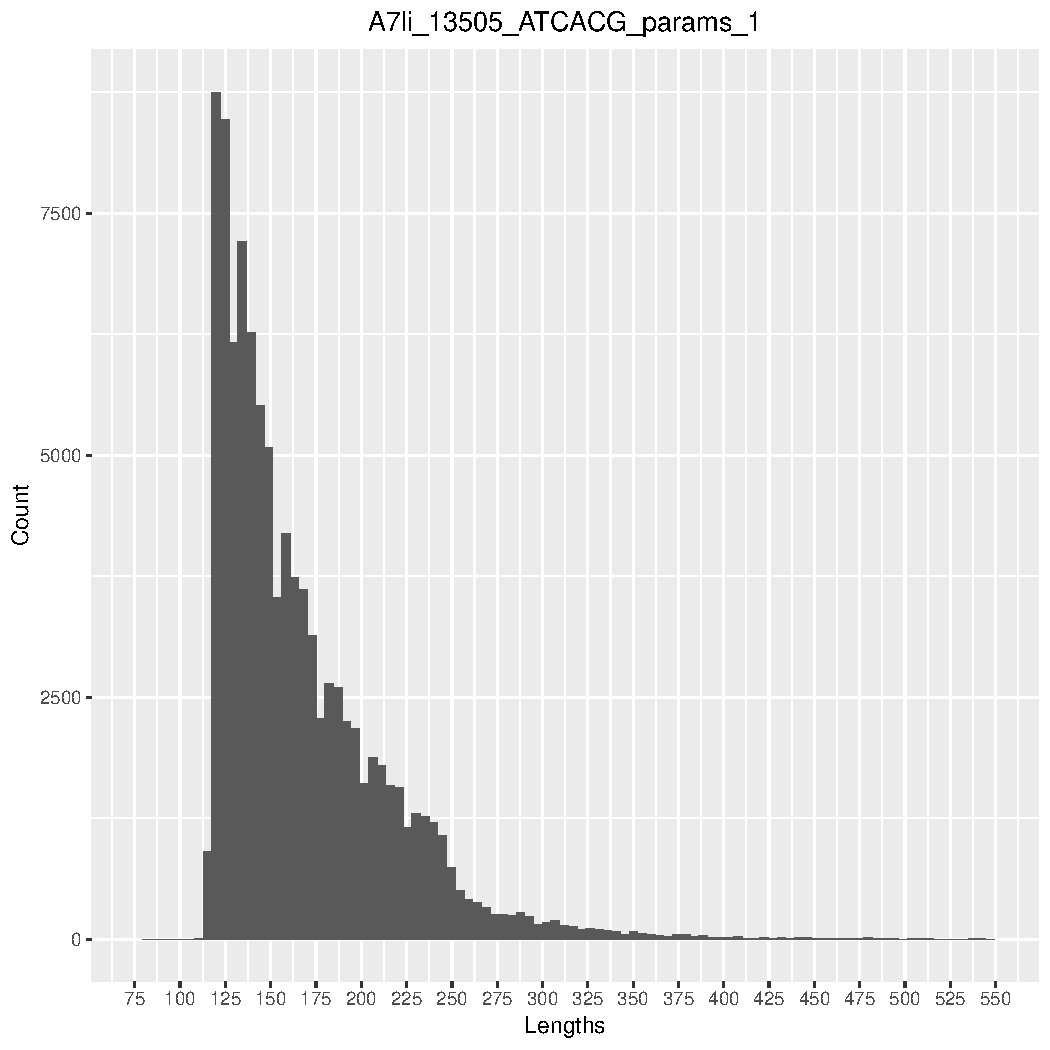
\includegraphics[width=\maxwidth]{figure/unnamed-chunk-4-1} 


\includegraphics[width=\maxwidth]{figure/unnamed-chunk-4-2} 
\begin{kframe}

{\ttfamily\noindent\color{warningcolor}{\#\# Warning: Removed 26 rows containing non-finite values (stat\_bin).}}

{\ttfamily\noindent\color{warningcolor}{\#\# Warning: Removed 1 rows containing missing values (geom\_bar).}}\end{kframe}
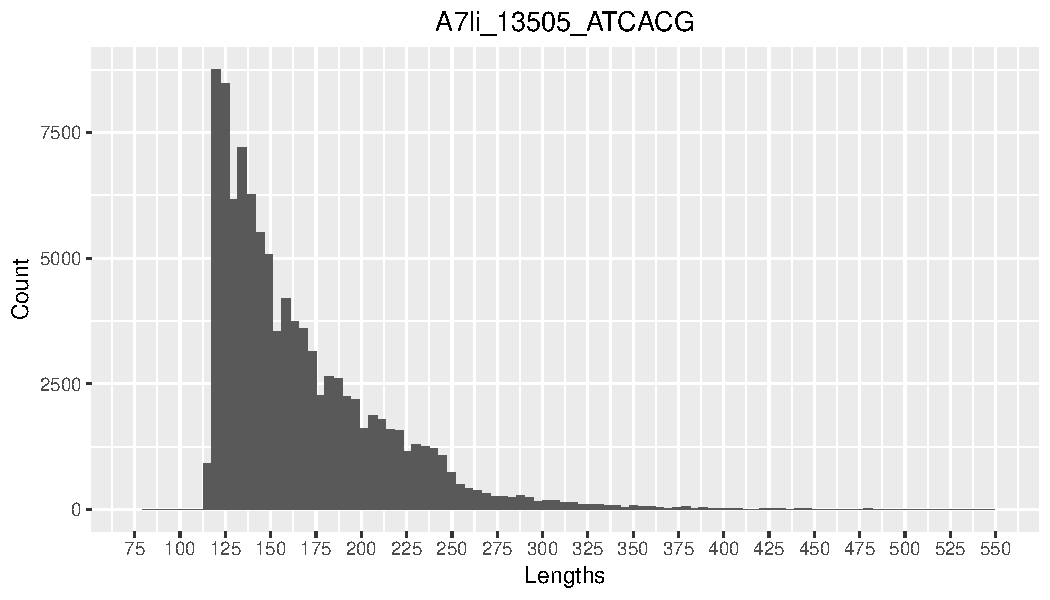
\includegraphics[width=\maxwidth]{figure/unnamed-chunk-4-3} 


\includegraphics[width=\maxwidth]{figure/unnamed-chunk-4-4} 
\begin{kframe}

{\ttfamily\noindent\color{warningcolor}{\#\# Warning: Removed 20 rows containing non-finite values (stat\_bin).}}

{\ttfamily\noindent\color{warningcolor}{\#\# Warning: Removed 1 rows containing missing values (geom\_bar).}}\end{kframe}
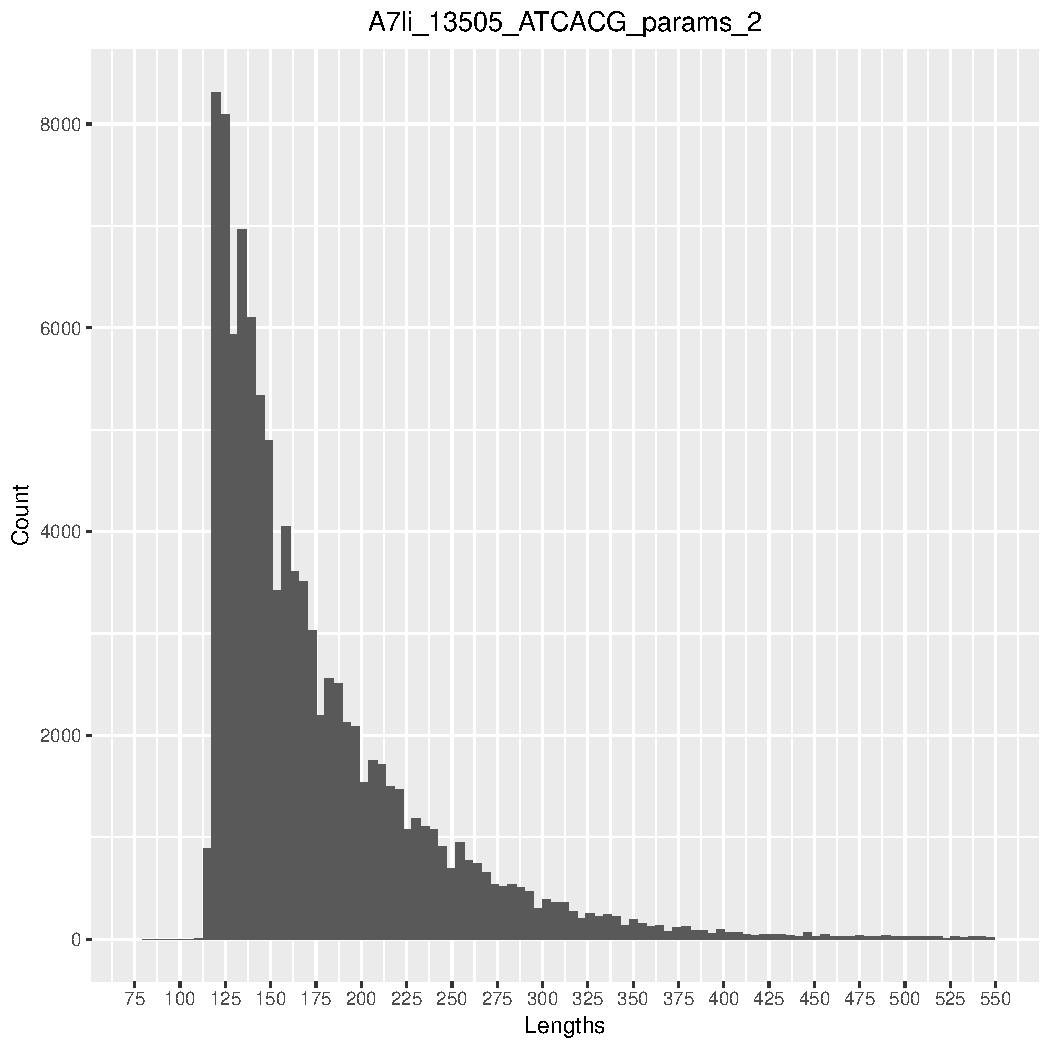
\includegraphics[width=\maxwidth]{figure/unnamed-chunk-4-5} 


\includegraphics[width=\maxwidth]{figure/unnamed-chunk-4-6} 
\begin{kframe}

{\ttfamily\noindent\color{warningcolor}{\#\# Warning: Removed 1 rows containing missing values (geom\_bar).}}\end{kframe}
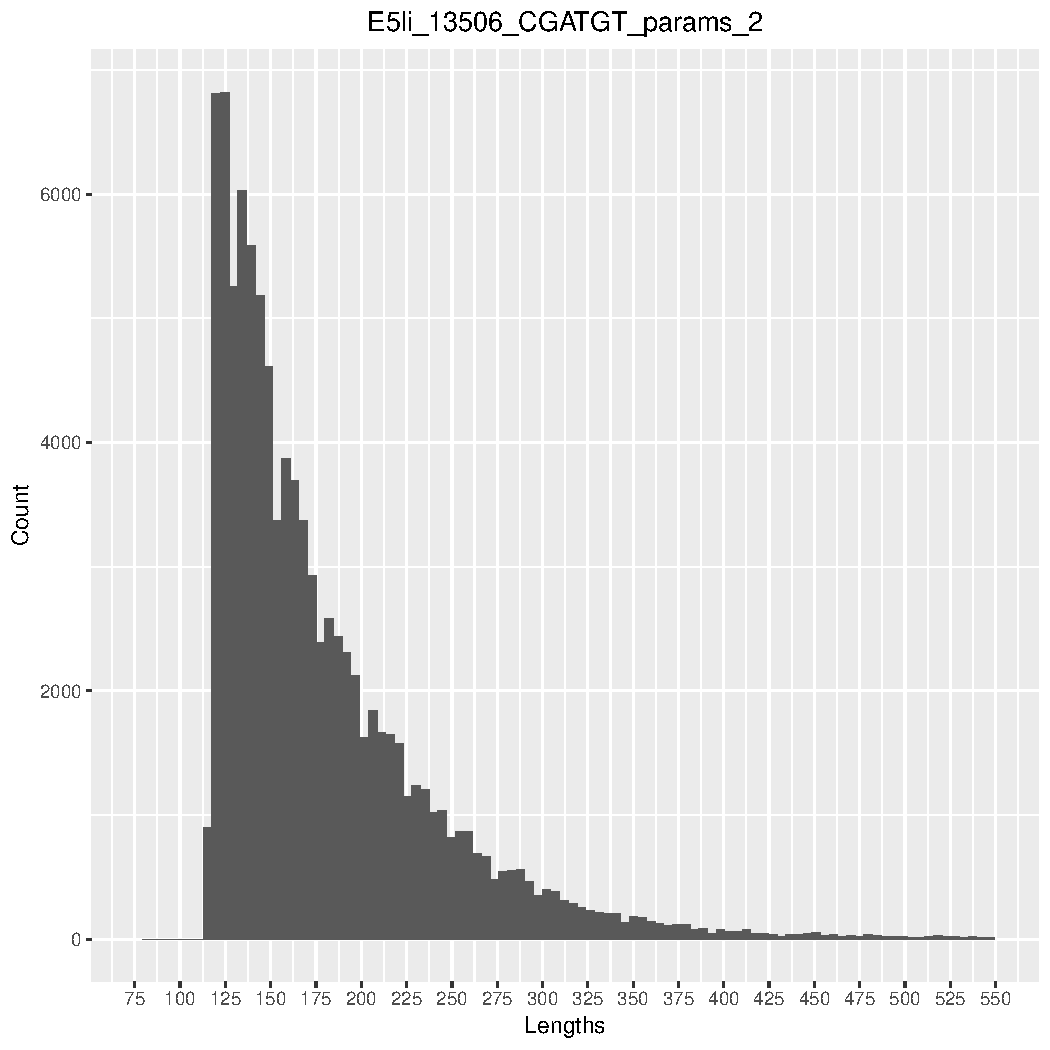
\includegraphics[width=\maxwidth]{figure/unnamed-chunk-4-7} 


\includegraphics[width=\maxwidth]{figure/unnamed-chunk-4-8} 
\begin{kframe}

{\ttfamily\noindent\color{warningcolor}{\#\# Warning: Removed 1242026 rows containing non-finite values (stat\_bin).}}

{\ttfamily\noindent\color{warningcolor}{\#\# Warning: Removed 1 rows containing missing values (geom\_bar).}}\end{kframe}
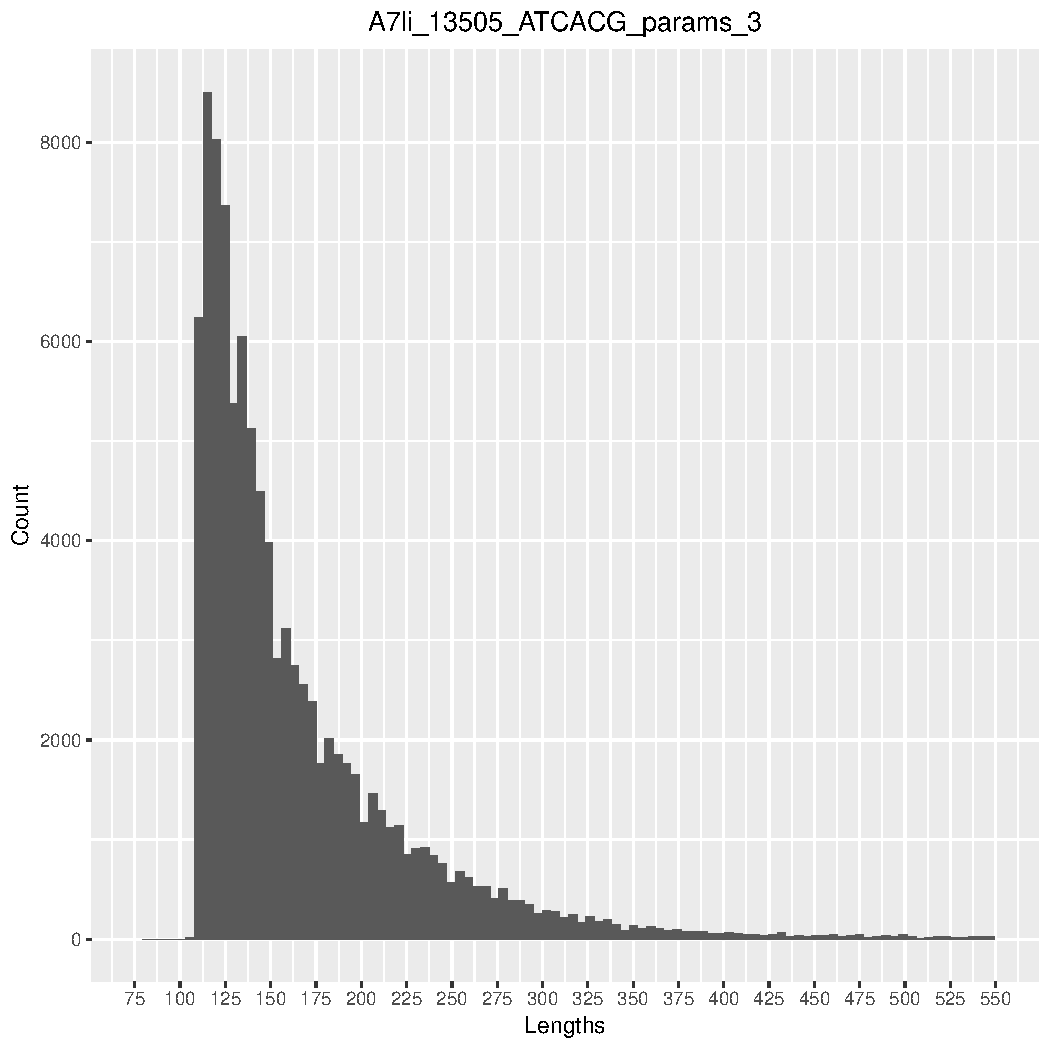
\includegraphics[width=\maxwidth]{figure/unnamed-chunk-4-9} 


\includegraphics[width=\maxwidth]{figure/unnamed-chunk-4-10} 
\begin{kframe}

{\ttfamily\noindent\color{warningcolor}{\#\# Warning: Removed 948769 rows containing non-finite values (stat\_bin).}}

{\ttfamily\noindent\color{warningcolor}{\#\# Warning: Removed 1 rows containing missing values (geom\_bar).}}\end{kframe}
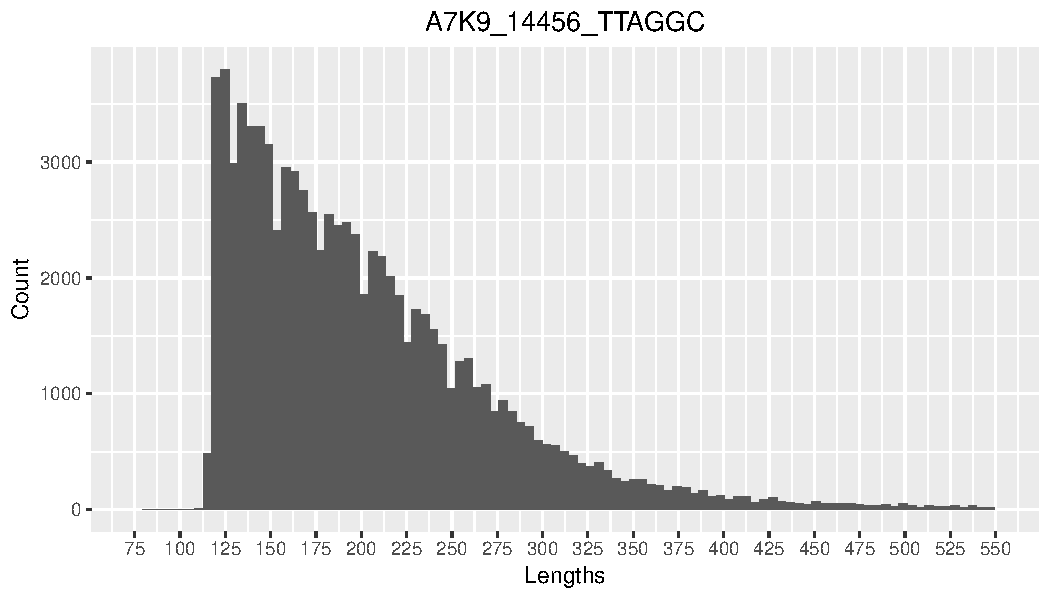
\includegraphics[width=\maxwidth]{figure/unnamed-chunk-4-11} 


\includegraphics[width=\maxwidth]{figure/unnamed-chunk-4-12} 
\begin{kframe}

{\ttfamily\noindent\color{warningcolor}{\#\# Warning: Removed 2966 rows containing non-finite values (stat\_bin).}}

{\ttfamily\noindent\color{warningcolor}{\#\# Warning: Removed 1 rows containing missing values (geom\_bar).}}\end{kframe}
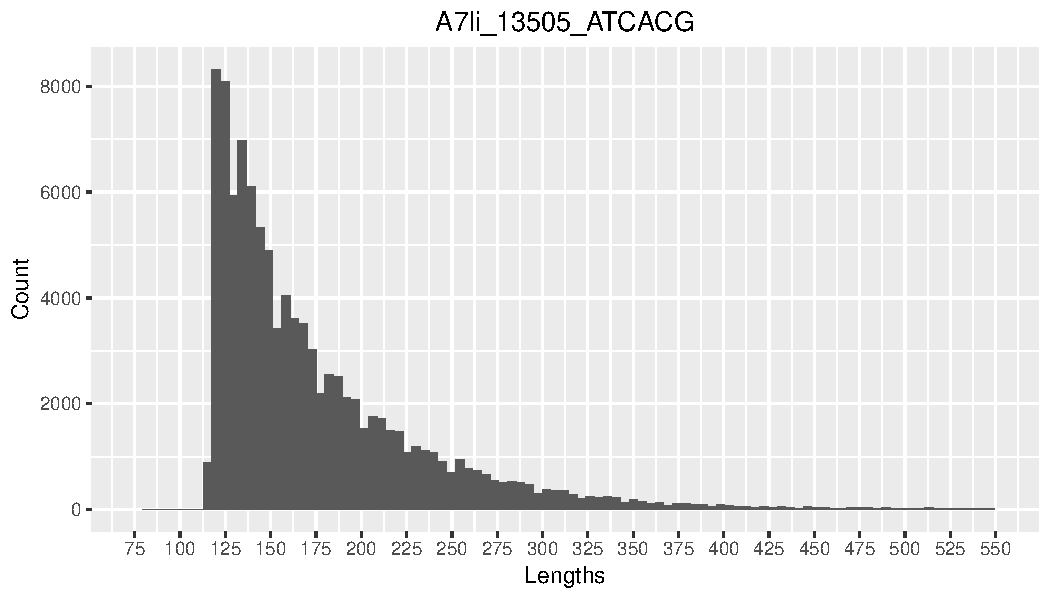
\includegraphics[width=\maxwidth]{figure/unnamed-chunk-4-13} 


\includegraphics[width=\maxwidth]{figure/unnamed-chunk-4-14} 
\begin{kframe}

{\ttfamily\noindent\color{warningcolor}{\#\# Warning: Removed 1542 rows containing non-finite values (stat\_bin).}}

{\ttfamily\noindent\color{warningcolor}{\#\# Warning: Removed 1 rows containing missing values (geom\_bar).}}\end{kframe}
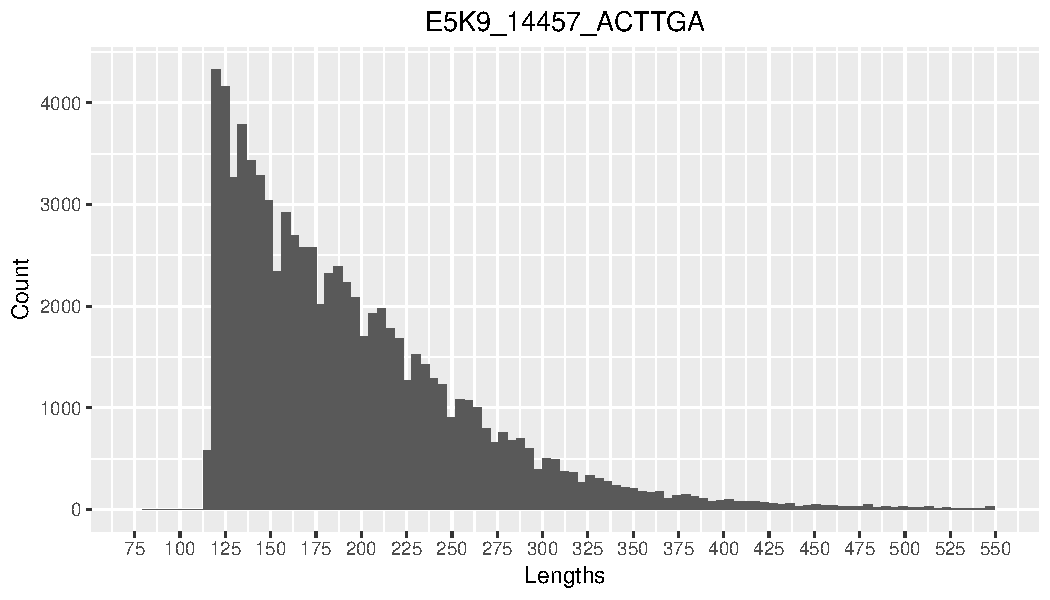
\includegraphics[width=\maxwidth]{figure/unnamed-chunk-4-15} 


\includegraphics[width=\maxwidth]{figure/unnamed-chunk-4-16} 
\begin{kframe}

{\ttfamily\noindent\color{warningcolor}{\#\# Warning: Removed 2 rows containing non-finite values (stat\_bin).}}

{\ttfamily\noindent\color{warningcolor}{\#\# Warning: Removed 1 rows containing missing values (geom\_bar).}}\end{kframe}
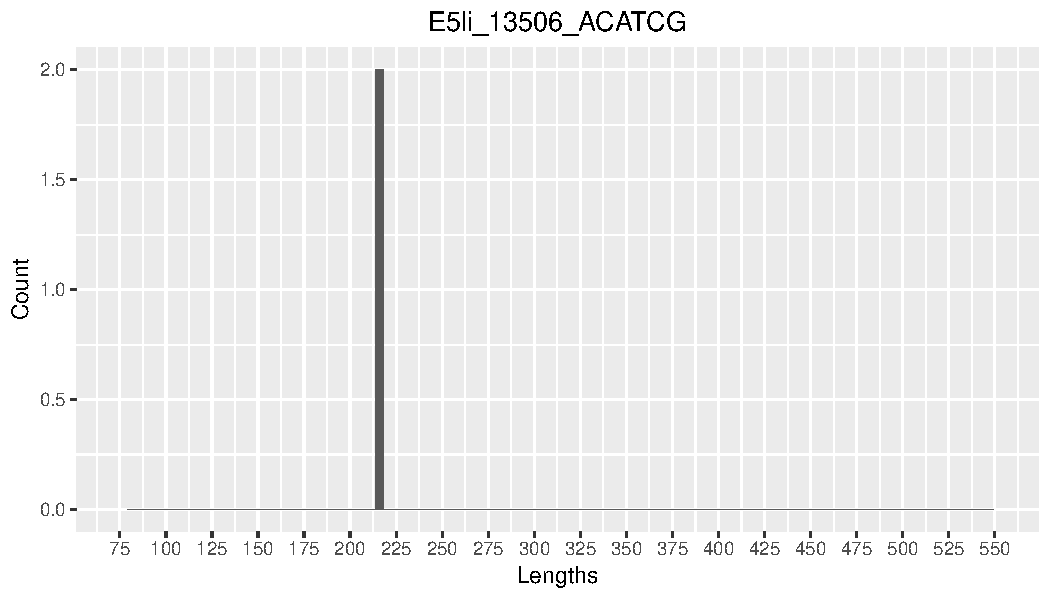
\includegraphics[width=\maxwidth]{figure/unnamed-chunk-4-17} 


\includegraphics[width=\maxwidth]{figure/unnamed-chunk-4-18} 
\begin{kframe}

{\ttfamily\noindent\color{warningcolor}{\#\# Warning: Removed 1244840 rows containing non-finite values (stat\_bin).}}

{\ttfamily\noindent\color{warningcolor}{\#\# Warning: Removed 1 rows containing missing values (geom\_bar).}}\end{kframe}
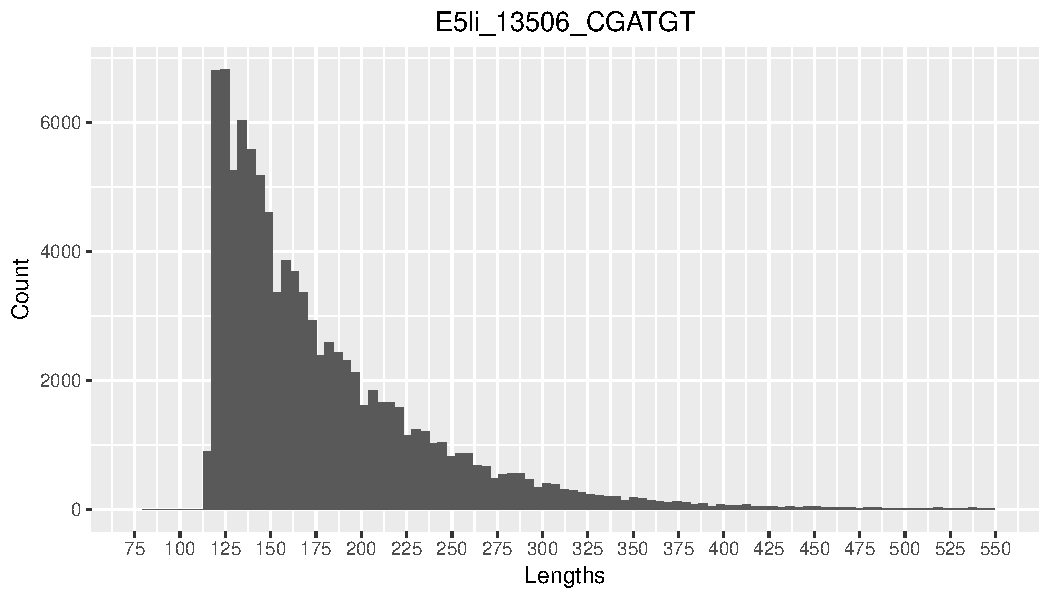
\includegraphics[width=\maxwidth]{figure/unnamed-chunk-4-19} 


\includegraphics[width=\maxwidth]{figure/unnamed-chunk-4-20} 
\begin{kframe}

{\ttfamily\noindent\color{warningcolor}{\#\# Warning: Removed 2216571 rows containing non-finite values (stat\_bin).}}

{\ttfamily\noindent\color{warningcolor}{\#\# Warning: Removed 1 rows containing missing values (geom\_bar).}}\end{kframe}
\includegraphics[width=\maxwidth]{figure/unnamed-chunk-4-21} 

\includegraphics[width=\maxwidth]{figure/unnamed-chunk-4-22} 
\begin{kframe}

{\ttfamily\noindent\color{warningcolor}{\#\# Warning: Removed 3892 rows containing non-finite values (stat\_bin).}}

{\ttfamily\noindent\color{warningcolor}{\#\# Warning: Removed 1 rows containing missing values (geom\_bar).}}\end{kframe}
\includegraphics[width=\maxwidth]{figure/unnamed-chunk-4-23} 

\includegraphics[width=\maxwidth]{figure/unnamed-chunk-4-24} 
\begin{kframe}

{\ttfamily\noindent\color{warningcolor}{\#\# Warning: Removed 268 rows containing non-finite values (stat\_bin).}}

{\ttfamily\noindent\color{warningcolor}{\#\# Warning: Removed 1 rows containing missing values (geom\_bar).}}\end{kframe}
\includegraphics[width=\maxwidth]{figure/unnamed-chunk-4-25} 

\includegraphics[width=\maxwidth]{figure/unnamed-chunk-4-26} 
\begin{kframe}

{\ttfamily\noindent\color{warningcolor}{\#\# Warning: Removed 1 rows containing missing values (geom\_bar).}}\end{kframe}
\includegraphics[width=\maxwidth]{figure/unnamed-chunk-4-27} 

\includegraphics[width=\maxwidth]{figure/unnamed-chunk-4-28} 
\begin{kframe}

{\ttfamily\noindent\color{warningcolor}{\#\# Warning: Removed 1888585 rows containing non-finite values (stat\_bin).}}

{\ttfamily\noindent\color{warningcolor}{\#\# Warning: Removed 1 rows containing missing values (geom\_bar).}}\end{kframe}
\includegraphics[width=\maxwidth]{figure/unnamed-chunk-4-29} 

\includegraphics[width=\maxwidth]{figure/unnamed-chunk-4-30} 

\end{knitrout}

\begin{knitrout}
\definecolor{shadecolor}{rgb}{0.969, 0.969, 0.969}\color{fgcolor}\begin{kframe}
\begin{alltt}
\hlstd{mapq} \hlkwb{<-} \hlkwd{read.csv2}\hlstd{(}\hlkwc{file} \hlstd{=} \hlstr{"/home/lucas/ISGlobal/TestSet/align_tests/params_1/A7K9_14456_TTAGGC_MAPQ.csv"}\hlstd{,} \hlkwc{sep} \hlstd{=} \hlstr{"\textbackslash{}t"}\hlstd{,} \hlkwc{header} \hlstd{=} \hlnum{FALSE}\hlstd{)}
\hlstd{df} \hlkwb{<-} \hlkwd{as.data.frame}\hlstd{(}\hlkwd{as.numeric}\hlstd{(mapq))}
\hlkwd{colnames}\hlstd{(df)} \hlkwb{<-} \hlstr{"MAPQ"}
\hlstd{title} \hlkwb{<-} \hlstr{"A7K9_14456_TTAGGC"}
\hlkwd{print}\hlstd{(}\hlkwd{ggplot}\hlstd{(df,} \hlkwd{aes}\hlstd{(}\hlkwc{x} \hlstd{= MAPQ))} \hlopt{+}
        \hlkwd{geom_histogram}\hlstd{(}\hlkwc{binwidth} \hlstd{=} \hlnum{1}\hlstd{)} \hlopt{+}
        \hlkwd{labs}\hlstd{(}\hlkwc{x} \hlstd{=} \hlstr{"MAPQ"}\hlstd{,} \hlkwc{y} \hlstd{=} \hlstr{"Count"}\hlstd{)} \hlopt{+}
        \hlkwd{ggtitle}\hlstd{(title)} \hlopt{+}
        \hlkwd{theme}\hlstd{(}\hlkwc{plot.title} \hlstd{=} \hlkwd{element_text}\hlstd{(}\hlkwc{hjust} \hlstd{=} \hlnum{0.5}\hlstd{))} \hlopt{+}
        \hlkwd{scale_x_continuous}\hlstd{(}\hlkwc{breaks} \hlstd{=} \hlkwd{seq}\hlstd{(}\hlnum{0}\hlstd{,} \hlnum{45}\hlstd{,} \hlkwc{by} \hlstd{=} \hlnum{2}\hlstd{),} \hlkwc{limits} \hlstd{=} \hlkwd{c}\hlstd{(}\hlnum{0}\hlstd{,}\hlnum{48}\hlstd{))} \hlopt{+}
        \hlkwd{scale_y_continuous}\hlstd{(}\hlkwc{breaks} \hlstd{=} \hlkwd{seq}\hlstd{(}\hlnum{0}\hlstd{,}\hlnum{80000}\hlstd{,} \hlkwc{by} \hlstd{=} \hlnum{5000}\hlstd{)))}
\end{alltt}
\end{kframe}\begin{figure}[h]
\includegraphics[width=\maxwidth]{figure/p3-1} \caption[Tralala]{Tralala}\label{fig:p3}
\end{figure}


\end{knitrout}


And some text after.
\end{document}
